\begin{name}
	{\tenchude}
	{\tendethi}
	{\tentruong}
	{\thoigian}
	\end{name}
\TN
\Opensolutionfile{ans}[ans/de7-ABCD]
\begin{ex}%[1D2H1-2]%Câu 1
	Cho dãy số $(u_n)$ với $u_n=\dfrac{2n}{3n+2}$, $n\in\mathbb{N}^*$. Khẳng định nào sau đây đúng?\vspace{3pt}
	\choice
	{$u_2=1$}
	{\True $u_2=\dfrac{1}{2}$}
	{$u_2=-\dfrac{1}{2}$}
	{$u_2=\dfrac{1}{3}$}
	\loigiai{
		Ta có $(u_n)$ với 
		$\begin{aligned}[t]
			u_n&=\dfrac{2n}{3n+2}, n\in\mathbb{N}^*.
		\end{aligned}$\\
	Suy ra $u_2=\dfrac{2\cdot2}{3\cdot2+2}=\dfrac{4}{8}=\dfrac{1}{2}$.
	}
\end{ex}
\begin{ex}%[2H5H2-3]%Câu 2
	Trong không gian $Oxyz$, cho đường thẳng $d\colon\dfrac{x-2}{2}=\dfrac{y+1}{-1}=\dfrac{z+2}{2}$. Đường thẳng $d$ đi qua điểm nào dưới đây?
	\choice
	{$A(2;-1;2)$}
	{$B(-2;1;2)$}
	{$C(2;1;2)$}
	{\True $D(2;-1;-2)$}
	\loigiai{
		Đường thẳng $d\colon\dfrac{x-2}{2}=\dfrac{y+1}{-1}=\dfrac{z+2}{2}=t$.\\
		Phương trình tham số $d\colon\heva{&x=2+3t\\ &y=-1-t\\ &z=-2+2t.}$\\
		Chọn $t=0$, đường thẳng $d$ đi qua điểm $D(2;-1;-2)$.
	}
\end{ex}
\begin{ex}%[1D6H2-2]%Câu 3
	Với $a$, $b$ là các số thực dương khác $1$ thỏa mãn $\log_a b=\dfrac{3}{2}$. Giá trị của biểu thức $\log_a b^4$ bằng\vspace{3pt}
	\choice
	{$\dfrac{8}{3}$}
	{$3$}
	{$\dfrac{4}{3}$}
	{\True $6$}
	\loigiai{
		Ta có $\log_ab^4=4\log_ab$.\\
		Mặt khác bài cho $\log_ab=\dfrac{3}{2}$.\\
		Suy ra $\log_ab^4=4\cdot\dfrac{3}{2}=6$.
	}
\end{ex}
\begin{ex}%[1H8H7-2]%Câu 4
	Cho khối chóp $S.ABCD$ có chiều cao bằng $5$, đáy $ABCD$ là hình bình hành có diện tích bằng $6$. Thể tích khối chóp $S.ABC$ bằng
	\choice
	{$10$}
	{$15$}
	{\True $5$}
	{$30$}
	\loigiai{
		Ta có công thức thể tích $V_{\text{chóp}}=\dfrac{1}{3}\cdot S_d\cdot h$.\\
		Suy ra $V_{S.ABC}=\dfrac{1}{3}\cdot S_{\triangle ABC}\cdot h$.\\
		Mặt khác ta có $S_{\triangle ABC}=\dfrac{1}{2}S_{ABCD}=\dfrac{1}{2}\cdot6=3$.\\
		Suy ra $V_{S.ABC}=\dfrac{1}{3}\cdot S_{\triangle ABC}\cdot h=\dfrac{1}{3}\cdot3\cdot5=5$.
	}
\end{ex}
\begin{ex}%[2H5H1-3]%Câu 5
	Trong không gian $Oxyz$, mặt phẳng $(\alpha)\colon x+2y+3z-6=0$ cắt trục tung tại điểm có tung độ bằng
	\choice
	{$2$}
	{$6$}
	{\True $3$}
	{$1$}
	\loigiai{
		Trong không gian $Oxyz$, mặt phẳng $(\alpha)\colon x+2y+3z-6=0$ cắt trục tung, suy ra mặt phẳng $(\alpha)$ sẽ cắt trục tung tại điểm $(0;a;0)$
		\begin{eqnarray*}
			 \Rightarrow 1\cdot0+2\cdot a+3\cdot0-6=0 \Leftrightarrow a=3.
		\end{eqnarray*}
	Vậy mặt phẳng $(\alpha)\colon x+2y+3z-6=0$ cắt trục tung tại điểm có tung độ bằng $3$.
	}
\end{ex}
\textbf{\textit{Sử dụng thông tin dưới đây để trả lời câu \ref{câu 6-đề 7} và câu \ref{câu 7-đề 7}}}\\[0.5em]
Cho hàm số $y=f(x)$ có bảng biến thiên như sau
\begin{center}
	
\begin{tikzpicture}
		\tikzset{double style/.append style={double distance=1.5pt}}
		\tkzTabInit[nocadre=false,lgt=1.2,espcl=2.5,deltacl=0.6]
		{$x$ /0.6,$y'$ /0.6,$y$ /2}
		{$-\infty$,$-2$,$3$,$+\infty$}
		\tkzTabLine{,+,d,-,$0$,+,}
		\tkzTabVar{-/$5$,+D+/$+\infty$/$4$,-/$0$,+/$+\infty$}
	\end{tikzpicture}
\end{center}
\begin{ex}%[2D1V3-1]%Câu 6
	\label{câu 6-đề 7}
	Giá trị nhỏ nhất của hàm số $y=f(x)$ trên đoạn $[0;6]$ bằng
	\choice
	{\True $0$}
	{$4$}
	{$f(4)$}
	{$f(6)$}
	\loigiai{
		Từ bảng biến thiên, ta thấy giá trị nhỏ nhất của hàm số $y=f(x)$ trên đoạn $\left[0;6\right]$ bằng $0$.
	}
\end{ex}
\begin{ex}%[2D1H4-1]%Câu 7
	\label{câu 7-đề 7}
	Tổng số đường tiệm cận đứng và tiệm cận ngang của đồ thị hàm số $y=f(x)$ là
	\choice
	{\True $2$}
	{$1$}
	{$3$}
	{$0$}
	\loigiai{
		Từ bảng biến thiên, ta có
		$
			\lim\limits_{x\to-\infty}y=5; \lim\limits_{x \to +\infty} y=+\infty
		$
		nên đồ thị hàm số $y=f(x)$ có một tiệm cận ngang.\\
		Ta lại có $\lim\limits_{x \to -2^-} y=+\infty$ nên đồ thị hàm số $y=f(x)$ có một tiệm cận đứng.\\
		Vậy tổng số đường tiệm cận đứng và tiệm cận ngang của đồ thị hàm số $y=f(x)$ là $2$.
	}
\end{ex}
\begin{ex}%[1D6H4-2]%Câu 8
	Tập nghiệm của bất phương trình $3^{2x-3}\le\dfrac{1}{3}$ là
	\choice
	{\True $(-\infty;1]$}
	{$[1;+\infty)$}
	{$(-\infty;2]$}
	{$[2;+\infty)$}
	\loigiai{
		Ta có 
		$\begin{aligned}[t]
			3^{2x-3}\leq\dfrac{1}{3}
			& \Leftrightarrow 3^{2x-3}\leq3^{-1}\\
			& \Leftrightarrow 2x-3\leq-1\\
			& \Leftrightarrow 2x\leq2\\
			& \Leftrightarrow x\leq1.
		\end{aligned}$\\
	Vậy tập nghiệm của bất phương trình là $\left(-\infty;1\right]$.
	}
\end{ex}

\begin{ex}%[2H2H1-2]%Câu 9
	% \immini[thm]{
		Cho hình lập phương $ABCD.A'B'C'D'$ có cạnh bằng $a$. Độ dài của vectơ $\overrightarrow{u}=\overrightarrow{A'C'}-\overrightarrow{A'A}$ bằng
	\choice
	{$\sqrt{2}a$}
	{$\dfrac{\sqrt{3}a}{2}$}
	{$\sqrt{6}a$}
	{\True $\sqrt{3}a$}
	% }{
	% 	\begin{tikzpicture}[line cap=round, line join=round, font=\footnotesize, thick]
	% 		\def\a{2.75}
	% 		\path 	(0:0) coordinate (A)
	% 				++(0:\a) coordinate (D)
	% 				++(-130:\a/2) coordinate (C)
	% 				($(A)+(C)-(D)$) coordinate (B)
	% 				($(A)+(90:\a)$) coordinate (A')
	% 				($(B)+(90:\a)$) coordinate (B')
	% 				($(C)+(90:\a)$) coordinate (C')
	% 				($(D)+(90:\a)$) coordinate (D');
	% 		\draw[dashed,thin] (B)--(A)--(D) (A)--(A');
	% 		\draw[thick] (C)--(C') (D)--(D') (B)--(B') (B)--(C)--(D) (A')--(B')--(C')--(D')--cycle;
	% 		\foreach \x/\y in {A/180,B/180,C/0,D/0,A'/180,B'/180,C'/0,D'/0}
	% 			\fill[black] (\x) circle (1pt) ($(\y:3mm)+(\x)$) node {$\x$};	
	% 	\end{tikzpicture}
	% }
	\loigiai{
		Theo qui tắc ba điểm, ta có $\overrightarrow{u} =\overrightarrow{A'C'}-\overrightarrow{A'A} =\overrightarrow{AC'}$.\\
		Suy ra độ dài $|\overrightarrow{u}| =\left|\overrightarrow{A'C'}-\overrightarrow{A'A}\right| =\left|\overrightarrow{AC'}\right| =AC'$.
		\immini{
			Có $ABCD.A'B'C'D'$ là hình lập phương cạnh $a$ và có $AC'$ là đường chéo của hình lập phương nên ta suy ra
			\begin{align*}
				AC'&=\sqrt{AC^2+CC'^2}=\sqrt{AB^2+AD^2+CC'^2} \\
				&=\sqrt{AB^2+AD^2+AA'^2}=\sqrt{a^2+a^2+a^2}=a\sqrt{3}.
			\end{align*}
		}{
			\begin{tikzpicture}[line cap=round, line join=round, font=\footnotesize, thick, blue, >=stealth]
				\def\a{2.75}
				\path 	(0:0) coordinate (A)
				++(0:\a) coordinate (D)
				++(-130:\a/2) coordinate (C)
				($(A)+(C)-(D)$) coordinate (B)
				($(A)+(90:\a)$) coordinate (A')
				($(B)+(90:\a)$) coordinate (B')
				($(C)+(90:\a)$) coordinate (C')
				($(D)+(90:\a)$) coordinate (D');
				\draw[dashed,thin,->,magenta] (A)--(A');
				\draw[dashed,thin,->,magenta] (A)--(B);
				\draw[dashed,thin,->,magenta] (A)--(D);
				\draw[thick] (C)--(C') (D)--(D') (B)--(B') (B)--(C)--(D) (A')--(B')--(C')--(D')--cycle;
				\foreach \x/\y in {A/180,B/180,C/0,D/0,A'/180,B'/180,C'/0,D'/0}
				\fill[black] (\x) circle (1pt) ($(\y:3mm)+(\x)$) node {$\x$};
				\draw[->,very thick,magenta] (A)--(C');
			\end{tikzpicture}
		}
		
	}
\end{ex}
\begin{ex}%[1D5H2-3]%Câu 10
	Một vườn thú ghi lại tuổi thọ (đơn vị: năm) của $20$ con hổ và thu được kết quả như sau
	\begin{center}
		\begin{tabular}{|c|c|c|c|c|c|}\hline
			Tuổi thọ & $[14;15)$ & $[15;16)$ & $[16;17)$ & $[17;18)$ & $[18;19)$ \\ \hline
			Số con hổ & $1$ & $3$ & $8$ & $6$ & $2$ \\ \hline
		\end{tabular}
	\end{center}
	Nhóm chứa tứ phân vị thứ nhất là
	\choice
	{$[14;15)$}
	{$[15;16)$}
	{\True $[16;17)$}
	{$[17;18)$}
	\loigiai{
		Số con hổ được khảo sát là $n=20$.\\
		Gọi $x_1,x_2,\ldots,x_{20}$ là tuổi thọ của $20$ con hổ được sắp xếp theo thứ tự không giảm.\\
		Ta có 
		$\begin{aligned}[t]
			x_1 & \in \left[14;15\right); \\
			x_2,x_3,x_4 & \in \left[15;16\right); \\
			x_5,x_6,\ldots,x_{12} & \in \left[16;17\right); \\
			x_{13},x_{14},\ldots,x_{18} & \in \left[17;18\right); \\
			x_{19},x_{20} & \in \left[18;19\right).
		\end{aligned}$\\
	Do đó đối với dãy số liệu $x_1, x_2, \ldots, x_{20}$ thì tứ phân vị thứ nhất của dãy số $x_1, x_2, \ldots, x_{20}$ là $\dfrac{1}{2}\left(x_5+x_6\right)$.\\
	Do đó $x_5, x_6$ thuộc nhóm $\left[16;17\right)$ nên tứ phân vị thứ nhất thuộc nhóm $\left[16;17\right)$.
	}
\end{ex}
\begin{ex}%[2D4V3-4]%Câu 11

		Cho hình phẳng $(H)$ giới hạn bởi đồ thị hàm số $y=4-x^2$ và trục hoành. Thể tích của khối tròn xoay được tạo thành khi quay $(H)$ xung quanh trục $Ox$ bằng\vspace{3pt}
	\choice
	{$\dfrac{32\pi}{3}$}
	{$\dfrac{512}{15}$}
	{\True $\dfrac{512\pi}{15}$}
	{$\dfrac{32}{3}$}
	
	\loigiai{
		\immini{
		Ta có phương trình hoành độ giao điểm của $y=4-x^2$ và trục hoành $y=0$
		$$4-x^2=0 \Leftrightarrow x=\pm2.$$
		Thể tích khối tròn xoay được tạo thành khi quay $(H)$ xung quanh trục $Ox$ là
		\begin{align*}
			V=\pi\displaystyle\int\limits_{-2}^2 \left(4-x^2\right)^2 \mathrm{\,d}x =\dfrac{512}{15}\pi.
		\end{align*}
		}{
		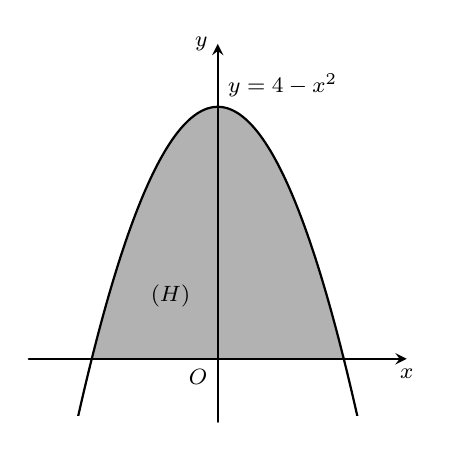
\begin{tikzpicture}[scale=0.8,>=stealth, font=\footnotesize, line join=round, line cap=round, thick]
			\def\a{-1} \def\b{0} \def\c{4} % Hệ số
			\def\xmin{-3} \def\xmax{3}
			\def\ymin{-1} \def\ymax{5}
			\fill[gray!60] plot[domain=-2:2](\x,{\a*(\x)^2+\b*(\x)+\c})--cycle;
			\draw[->] (\xmin,0)--(\xmax,0) node [below]{$x$};
			\draw[->] (0,\ymin)--(0,\ymax) node [left]{$y$};
			\node at (0,0) [below left]{$O$};
			\clip (\xmin+0.1,\ymin+0.1) rectangle (\xmax-0.1,\ymax-0.1);
			\draw[smooth,samples=300] plot(\x,{\a*(\x)^2+\b*(\x)+\c});
			\draw (0,4)node[above right]{$y=4-x^2$} (-0.75,1)node[]{$(H)$};
		\end{tikzpicture}
	}
	}
\end{ex}
\begin{ex}%[2D4H1-2]%Câu 12
	Cho hàm số $f(x)$ liên tục trên $\mathbb{R}$. Biết $F(x)$ là nguyên hàm của hàm số $f(x)$ thỏa mãn $F(2)=2$ và $F(x)=\displaystyle\int \left[x-f(x)\right] \mathrm{\,d}x$, $\forall x\in\mathbb{R}$, Giá trị của $F(4)$ bằng
	\choice
	{\True $5$}
	{$6$}
	{$8$}
	{$9$}
	\loigiai{
		Ta có 
		$\begin{aligned}[t]
			F(x)=\displaystyle\int x \mathrm{\,d}x -\displaystyle\int f(x) \mathrm{\,d}x
			=\dfrac{x^2}{2}+C-F(x) \Leftrightarrow 2F(x) =\dfrac{x^2}{2}+C.
		\end{aligned}$\\
	Tại $x=2$ ta có $2F(2)=2+C \Leftrightarrow C=2$.\\
	Suy ra $x=4$ ta được $2F(4)=\dfrac{4^2}{2}+C \Leftrightarrow 2F(4)=\dfrac{4^2}{2}+2 \Leftrightarrow 2F(4)=10 \Leftrightarrow F(4)=5$.
	}
\end{ex}

\Closesolutionfile{ans}

\inputansbox{6}{ans/de7-ABCD}

\TNTF

\Opensolutionfile{ans}[ans/de7-DS]

\begin{ex}%[1D7H2-1]%Câu 1
	Cho hàm số $f(x)=\ln\left(x^2-2x+1\right)-x$. Xét tính đúng sai của các mệnh đề sau
	\choiceTF
	{Tập xác định của hàm số là $\mathscr{D}=\mathbb{R}$}
	{\True Đạo hàm của hàm số $f(x)$ trên tập xác định của nó là $f'(x)=\dfrac{2}{x-1}-1$}
	{\True Số nghiệm của phương trình $f'(x)=0$ trên khoảng $(1;+\infty)$ là $1$}
	{Giá trị cực đại của $f(x)$ trên khoảng $(1;+\infty)$ là $a\ln 2+b$ với $a$, $b\in\mathbb{Z}$ thì $a+b=1$}
	\loigiai{
		\begin{itemchoice}
			\itemch Điều kiện $x^2-2x+1>0 \Leftrightarrow (x-1)^2>0 \Leftrightarrow x\ne1$.\\
			Suy ra tập xác định của hàm số là $\mathscr{D}=\mathbb{R}\setminus\{1\}$.
			\itemch Áp dụng công thức $\left(\ln u\right)'=\dfrac{u'}{u}$.\\
			Ta có $f(x)=\ln\left(x^2-2x+1\right)-x $.\\
			$\Rightarrow f'(x)=\dfrac{(x^2-2x+1)'}{x^2-2x+1}-1 =\dfrac{2x-2}{x^2-2x+1}-1 =\dfrac{2(x-1)}{(x-1)^2}-1 =\dfrac{2}{x-1}-1$.
			\itemch Ta có $f'(x)=0 \Leftrightarrow \dfrac{2}{x-1}-1=0 \Leftrightarrow x-1=2 \Leftrightarrow x=3$.\\
			Suy ra $f'(x)=0$ có nghiệm duy nhất.
			\itemch Lập bảng biến thiên $ \Rightarrow x=3$ là điểm cực đại của hàm số.\\
			Do đó $y_{CD}=f(3)=\ln4-3=2\ln2-3=a\ln2+b$.\\
			Suy ra $a=2, b=-3$ nên $a+b=2+(-3)=-1$.
		\end{itemchoice}
	}
\end{ex}

\begin{ex}%[2D5V1-2]%[2D5V1-3]%Câu 2
	Một nhà máy sản xuất bóng đèn có tỷ lệ bóng đèn đạt tiêu chuẩn là $82\%$. Trước khi xuất ra thị trường, mỗi bóng đèn được sản xuất ra đều phải qua một khâu kiểm tra chất lượng tự động. Vì sự kiểm tra này không chính xác tuyệt đối nên một bóng đèn tốt chỉ có xác suất $92\%$ được công nhận và một bóng đèn hỏng có xác suất $96\%$ được loại bỏ.
	\begin{itemize}
		\item Gọi $A$ là biến cố \lq\lq Bóng được công nhận đạt tiêu chuẩn sau khi qua kiểm tra chất lượng\rq\rq.
		\item Gọi $B$ là biến cố \lq\lq Sản phẩm đạt tiêu chuẩn\rq\rq.
	\end{itemize}
	Xét tính đúng sai của các mệnh đề sau
	\choiceTF[t]
	{$\mathrm{P}(B)=0{,}18$ ; $\mathrm{P}(\overline{B})=0{,}82$}
	{Xác suất có điều kiện $\mathrm{P}(A|\overline{B})=0{,}92$}
	{\True Tỉ lệ bóng được công nhận đạt tiêu chuẩn sau khi qua kiểm tra chất lượng là $76{,}16\%$}
	{Tỷ lệ bóng đèn tốt trong số những bóng đèn được công nhận là $98{,}01\%$ (kết quả làm tròn đến hàng phần trăm)}
	\loigiai{
		\textbf{Chú ý:} Bóng đèn đạt tiêu chuẩn là bóng đèn tốt và bóng đèn không đạt tiêu chuẩn là bóng đèn hỏng.
		\begin{itemchoice}
			\itemch Theo bài ra ta có $\mathrm{P}(B)=0{,}82$; $\mathrm{P}(\overline{B})=1-0{,}82=0{,}18$.
			\itemch Do tỉ lệ công nhận bóng đèn đạt tiêu chuẩn là $0{,}92$ nên $\mathrm{P}(A|B)=0{,92}$.\\
			Tie lệ loại bỏ một bóng đèn hỏng là $0{,}96$ nên $\mathrm{P}(A|\overline{B})=1-0{,}92=0{,}04$.\\
			Theo sơ đồ hình cây
			\itemch Theo công thức xác suất toàn phần ta có $$\mathrm{P}(A)=\mathrm{P}(B)\cdot\mathrm{P}(A|B)+\mathrm{P}(\overline{B})\cdot\mathrm{P}(A|\overline{B}) =0{82\cdot0{,}92}+0{,}18\cdot0{,}04 =0{,}7616.$$
			\itemch Tỉ lệ bóng đèn tốt trong số những bóng đèn được công nhận là $$\dfrac{0{,}82\cdot0{,}92}{0{,}82\cdot0{,}92+0{,}18\cdot0{,}04}=99{,}05.$$
		\end{itemchoice}
	}
\end{ex}

\begin{ex}%[2H2C2-6]%Câu 3
	\immini[thm]{
		Xét hai chiếc khinh khí cầu bay lên từ cùng một điểm trong cùng một ngày. Lúc $9$ giờ sáng, chiếc thứ nhất đang ở vị trí $A$ cách điểm xuất phát $2$ km về phía nam và $1$ km về phía đông, đồng thời cách mặt đất $0{,}5$ km. Chiếc thứ hai đang ở vị trí $B$ nằm cách điểm xuất phát $1$ km về phía bắc và $1{,}5$ km về phía tây đồng thời cách mặt đất $0{,}8$ km. Chọn hệ trục tọa độ $Oxyz$ với gốc $O$ đặt tại điểm xuất phát của hai khinh khí cầu, mặt phẳng $(Oxy)$ trùn với mặt đất, trục $Ox$ hướng về phía nam, trục $Oy$ hướng về phía đông và trục $Oz$ hướng thẳng đứng lên trời (như hình vẽ). Lấy đơn vị đo trên mỗi trục là km.
	}{\begin{tikzpicture}[scale=1,font=\footnotesize,>=stealth, line join=round, line cap=round]
		\def\xmin{-2} \def\xmax{4}
		\def\ymin{-2} \def\ymax{2}
		\def\zmax{3}
		\draw[->] (\xmin,0)--(\xmax,0) node [below]{$x$};
		\draw[->] (\ymax,\ymax)--(\ymin,\ymin)node [above]{$y$};
		\draw[->] (0,0)--(0,\zmax) node [left]{$z$};
		\draw (\xmax,0)node[above]{Nam} (\xmin,0)node[above]{Bắc} (\ymax,\ymax)node[above]{Tây} (\ymin,\ymin)node[below]{Đông};
		\node at (0,0) [below]{$O$};
		\coordinate (O) at (0,0);
		\coordinate (E) at (3,0);
		\coordinate (F) at (-1,-1);
		\coordinate (G) at ($(E)+(F)-(O)$);
		\coordinate (A) at ($(G)+(0,1.7)$);
		\draw[dashed] (F)--(G)--(E) (O)--(G) (O)--(A)node[above,blue,font=\fontsize{25pt}{2pt}\selectfont]{\faFly}--(G);
		\fill (A)circle(2pt);
		\coordinate (M) at (-1.5,0);
		\coordinate (N) at (0.5,0.5);
		\coordinate (P) at ($(M)+(N)-(O)$);
		\coordinate (B) at ($(P)+(0,1.5)$);
		\draw[dashed] (M)--(P)--(N) (O)--(P) (O)--(B)node[above,magenta,font=\fontsize{25pt}{2pt}\selectfont]{\faFly}--(P);
		\fill (B)circle(2pt);
	\end{tikzpicture}}
	\choiceTF
	{\True Tọa độ của khinh khí cầu thứ nhất lúc $9$ giờ sáng là $A(2;1;0{,}5)$}
	{Phương trình chính tắc của đường thẳng $AB$ là $\dfrac{x-2}{30}=\dfrac{y-1}{25}=\dfrac{z-0{,}5}{3}$}
	{\True Lúc $9$ giờ sáng, khoảng cách giữa hai chiếc khinh khí cầu là $3{,}92$ km (làm tròn đến hàng phần trăm)}
	{Từ $9$ giờ sáng đến $9$ giờ $10$ phút sáng, khinh khí cầu thứ nhất đi thẳng về hướng Nam với vận tốc $50$ km/h và độ cao không đổi để đến điểm $M$, khinh khí cầu thứ hai chuyển động thẳng đến điểm $N$ với vận tốc $60$ km/h, biết vectơ $\overrightarrow{BN}$ cùng hướng với vectơ $\overrightarrow{u}=(2;2;1)$. Bỏ qua lực cản của gió, khoảng cách $MN$ là $4{,}66$ km (làm tròn đến hàng phần trăm)}
	\loigiai{
		\begin{itemchoice}
			\itemch Vị trí của khinh khí cầu thứ nhất lúc $9$ giờ sáng là $A(x_A;y_A;z_A)$ biết
			\begin{itemize}
				\item $A$ cách điểm xuất phát $2$ km về phía Nam $ \Rightarrow x_A=2$.
				\item $1$ km về phía Đông $ \Rightarrow y_A=1$.
				\item Cách mặt đất $0{,}5$ km $ \Rightarrow z_A=0{,}5$.
			\end{itemize}
		Vậy $A(2;1;0{,}5)$.
			\itemch Dựa vào giả thiết, ta có $B(-1;-1{,}5;0{,}8)$.\\
			Suy ra $\overrightarrow{AB}=(-3;-2{,}5;0{,3})$.\\
			Đường thẳng $AB$ đi qua điểm $A(2;1;0{,}5)$ và có vec-tơ chỉ phương $\overrightarrow{u}=(30;25;-3)$ có phương trình chính tắc là $\dfrac{x-2}{30}=\dfrac{y-1}{25}=\dfrac{x-0{,}5}{-3}$.
			\itemch Lúc $9$ giờ sáng, khoảng cách giữa hai kinh khí cầu bằng $$AB=\sqrt{(-3)^2+(-2{,}5)^2+(0{,}3)^2}\approx3{,}92\, (\rm km).$$
			\itemch Để tính được khoảng cách $MN$ ta cần tìm được toạ độ của điểm $M$ và $N$ lúc $9$ giờ $10$ phút sáng
			\begin{itemize}
				\item Tìm điểm $M(x_M;y_M;z_M)$.\\
				Ta có khinh khí cầu thứ nhất di chuyển thẳng đều về phía Nam (tức hoành độ của khinh khí cầu không đổi $ \Leftrightarrow y_M=1$) với vận tốc $50\,\rm km/h$ suy ra từ $9$ giờ sáng đến $9$ giờ $10$ phút sáng, khinh khí cầu đi được $50\cdot\dfrac{1}{6}=\dfrac{25}{3}$ (km).\\
				$ \Rightarrow x_M=2+\dfrac{25}{3}=\dfrac{31}{3}$.\\
				Và cao độ không đổi $ \Rightarrow z_M=0{,}5$.\\
				Vậy điểm $M(\dfrac{31}{3};1;0{,}5)$.
				\item Tìm điểm $N(x_N;y_N;z_N)$\\
				Vì vectơ $\overrightarrow{BN}$ cùng hướng với vectơ $\overrightarrow{u}$ nên suy ra $\overrightarrow{BN}=k(2;2;1)\, (k>0)$.\\
				Khinh khí cầu thứ hai chuyển động thẳng đều đến điểm $N$ với vận tốc $60\, \rm km/h$, nên trong khoảng thời gian từ $9$ giờ sáng đến $9$ giờ $10$ phút sáng khinh khí cầu đi được $1$ đoạn $BN=60\cdot\dfrac{1}{6}=10 \Leftrightarrow k|(2;2;1)|=10 \Leftrightarrow k\sqrt{2^2+2^1+1^1}=10 \Leftrightarrow k=\dfrac{10}{3}$.\\
				$\overrightarrow{BN}=\left(x_N+1;y_N+1;z_N-0{,}8\right) =\dfrac{10}{3}(2;2;1) =\left(\dfrac{20}{3};\dfrac{20}{3};\dfrac{10}{3}\right) \Rightarrow \heva{&x_N=\dfrac{17}{3}\\ &y_N=\dfrac{31}{6}\\ &z_N=\dfrac{62}{15}.}$\\
				$ \Rightarrow N\left(\dfrac{17}{3};\dfrac{31}{3};\dfrac{62}{15}\right)$.\\
				Suy ra $MN=\sqrt{\left(\dfrac{17}{3}-\dfrac{31}{3}\right)^2+\left(\dfrac{31}{3}-1\right)^2+\left(\dfrac{62}{15}-0{,}5\right)^2} \approx 7{,}23$.
			\end{itemize}
		\end{itemchoice}
	}
\end{ex}

\begin{ex}%[2D4C3-2]%Câu 4
	\immini[thm]{
		Hình vẽ bên mô tả hiệu suất làm việc của hai công nhân trong một nhà máy trong thời gian $6$ giờ. Công nhân $A$ đang sản xuất với hiệu suất $Q'_1(t)=-2t^2+4t+58$ sản phẩm mỗi giờ, trong khi công nhân $B$ đang sản xuất với hiệu suất $Q'_2(t)=53+at$ sản phẩm mỗi giờ $(a\in\mathbb{R})$. Biết rằng hàm $Q_1(t)$ và $Q_2(t)$ mô phỏng số lượng sản phẩm mới làm được của công nhân $A$ và công nhân $B$ sau $t$ giờ. Xét tính đúng sai của các mệnh đề sau
	}{
		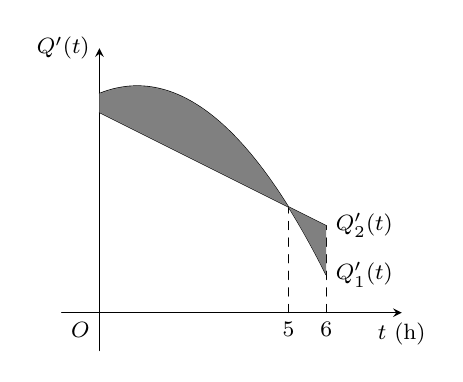
\begin{tikzpicture}[>=stealth, font=\footnotesize, line join=round, line cap=round,xscale=1,yscale=0.1,scale=0.48]
			\def\xmin{-1} \def\xmax{8}
			\def\ymin{-10} \def\ymax{70}
			\draw[->] (\xmin,0)--(\xmax,0) node [below]{$t$ (h)};
			\draw[->] (0,\ymin)--(0,\ymax) node [left]{$Q'(t)$};
			\node at (0,0) [below left]{$O$};
			\draw[dashed] (5,0)node[below]{$5$}--(5,28) (6,0)node[below]{$6$}--(6,10)node[right]{$Q'_1(t)$}--(6,23)node[right]{$Q'_2(t)$};
			\clip (\xmin+0.1,\ymin+0.1) rectangle (\xmax-0.5,\ymax-0.1);
			\draw[smooth,samples=300,domain=0:6] plot(\x,{-2*(\x)^2+4*(\x)+58});
			\draw[smooth,samples=300,domain=0:6] plot(\x,{-5*(\x)+53});
			\fill[gray] plot[domain=0:6](\x,{-2*(\x)^2+4*(\x)+58})--plot[domain=6:0](\x,{-5*(\x)+53})--cycle;
		\end{tikzpicture}
	}
	\choiceTF
	{\True Hiệu suất cực đại của công nhân $A$ là $60$ sản phẩm mỗi giờ}
	{Phần diện tích tô đậm biểu diễn cho tổng số lượng sản phẩm mới mà $2$ công nhân làm được trong $6$ giờ}
	{\True Sau $5$ giờ số lượng sản phẩm mới mà công nhân $A$ hoàn thành nhiều hơn công nhân $B$ là $54$ sản phẩm (kết quả làm tròn đến hàng đơn vị)}
	{Sau $6$ giờ làm việc tổng số lượng sản phẩm mới mà $2$ công nhân hoàn thành là $502$ sản phẩm}
	\loigiai{
		\begin{itemchoice}
			\itemch Ta có hiệu suất của công nhân $A$ là\\ $Q_1'(t)=-2t^2+4t+58 =-2(t^2-2t+1)+2+58 =-2(t-1)^2+60 \leq60$, $\forall t\in\left[0;6\right]$.\\
			Dấu \lq\lq$=$\rq\rq\, xảy ra khi $t=1$.\\
			Vậy hiệu suất cực đại của công nhân $A$ là $60$ sản phẩm mỗi giờ.
			\itemch Diện tích tô đậm bằng $\displaystyle\int\limits_0^6 \big|Q_1'-Q_2'\big| \mathrm{\,d}t$ nên nó không biểu diễn cho tổng số lượng sản phẩm mới mà 2 công nhân làm được trong $6$ giờ.
			\itemch Dựa vào biểu đồ, ta có 
			$$\begin{aligned}[t]
				Q_1'(5)=Q_2'(5) & \Leftrightarrow -2\cdot5^2+4\cdot5+58=53+5a\\
				& \Leftrightarrow a=-5.
			\end{aligned}$$
		Suy ra $Q_2'(5)=53-5t$.\\
		Sau 5 giờ, số lượng sản phẩm mới của công nhân $A$ hoàn thành nhiều hơn số lượng sản phẩm mới của công nhân $B$ bằng 
		\begin{align*}
			\displaystyle\int\limits_0^5 Q_1'(t) \mathrm{\,d}t -\displaystyle\int\limits_0^5 Q_2'(t) \mathrm{\,d}t =\displaystyle\int\limits_0^5 (-2t^2+4t+58) \mathrm{\,d}t -\displaystyle\int\limits_0^5 (53-5t) \mathrm{\,d}t =\dfrac{325}{6} \approx 54.
		\end{align*}
			\itemch Sau $6$ giờ làm việc tổng số lượng sản phẩm mới 2 công nhân hoàn thành bằng 
		\begin{align*}
			\displaystyle\int\limits_0^5 Q_1'(t) \mathrm{\,d}t +\displaystyle\int\limits_0^5 Q_2'(t) \mathrm{\,d}t =\displaystyle\int\limits_0^5 (-2t^2+4t+58) \mathrm{\,d}t +\displaystyle\int\limits_0^5 (53-5t) \mathrm{\,d}t =\dfrac{770}{3}+\dfrac{405}{2}= \dfrac{2755}{6} \approx 459.
		\end{align*}
		\end{itemchoice}
	}
\end{ex}

\Closesolutionfile{ans}

\inputansbox{3}{ans/de7-DS}

\TNSA

\Opensolutionfile{ans}[ans/de7-KQ]

\begin{ex}%[1H8V6-2]%Câu 1
	Cho hình chóp tam giác đều $S.ABC$ có $AB=2$, $SA=3$. Gọi $\alpha$ là số đo của góc nhị diện $[S,BC,A]$. Giá trị $\tan\alpha$ bằng bao nhiêu? (làm tròn kết quả đến hàng phần mười).
	\shortans[oly]{$4{,}8$}
	\loigiai{
		\begin{center}		
			\begin{tikzpicture}[line cap=round, line join=round, font=\footnotesize, thick, blue]
				\def\a{5} \def\h{3.5}
				\path 	(0:0) coordinate (A)
						(-45:2) coordinate (B)
						(0:\a) coordinate (C)
						($(C)!0.5!(B)$) coordinate (H)
						($(A)!2/3!(H)$) coordinate (O)
						($(O)+(90:\h)$) coordinate (S);
				\draw[] (S)--(A)--(B)--(C)--cycle (B)--(S)--(H);
				\draw[dashed,thin] (C)--(A)--(H) (S)--(O);
				\foreach \x/\y in {A/180,B/-90,C/0,H/-60,O/-90,S/90}
				\fill (\x) circle (1pt) ($(\x)+(\y:3mm)$) node {$\x$};
				\pic[draw,angle radius=2.5mm] {right angle=A--H--B};
				\pic[draw,angle radius=2mm] {right angle=S--O--H};
				\path (A)--(B) node[below,midway]{$2$}
				(A)--(S) node[left,midway]{$3$};
			\end{tikzpicture}
		\end{center}
	Kẻ $AH\perp BC$ (1)\\
	Gọi $O$ là tâm của $\triangle ABC$.\\
	Suy ra $SO\perp(ABC)$ (theo tính chất của hình chóp đều).\\
	$ \Rightarrow SO\perp BC$ (2)\\
	Từ (1) và (2) suy ra $BC\perp(SHA)$ $ \Rightarrow \left[S,BC,A\right] =\widehat{SHO}$.\\
	Vì $\triangle ABC$ đều nên ta có $AH=\sqrt{3} \Rightarrow \heva{&OH=\dfrac{\sqrt{3}}{3}\\ &AO=\dfrac{2\sqrt{3}}{3}.}$\\
	Suy ra $SO=\sqrt{3^2-\left(\dfrac{2\sqrt{3}}{3}\right)^2} =\dfrac{\sqrt{69}}{3}$.\\
	$ \Rightarrow \tan\alpha=\tan\widehat{SHO}=\dfrac{SO}{OH}=\dfrac{\sqrt{69}}{3}\div\dfrac{\sqrt{3}}{3} =\sqrt{23} \approx 4{,8}$.
	}
\end{ex}

\begin{ex}%[2D5V1-4]%Câu 2
	Một hộp đựng $12$ bóng đèn, các bóng đèn trong cùng hộp thì cùng màu. Số hộp đựng bóng đèn màu xanh nhiều gấp $9$ lần số hộp đựng bóng đèn màu vàng. Trong mỗi hộp đựng bóng đèn màu xanh có $3$ bóng bị hỏng, mỗi hộp đựng bóng đèn màu vàng có $2$ bóng bị hỏng. Tính xác suất để lấy ra hai bóng đèn màu xanh ở cùng một hộp, biết cả hai bóng đều bị hỏng. Viết kết quả làm tròn đến hàng phần trăm.
	\shortans[oly]{$0{,}96$}
	\loigiai{
		Gọi $A_1$ là biến cố lấy được một hộp đựng bóng đèn màu vàng.\\
		Suy ra $\mathrm{P}(A_1)=\dfrac{1}{1+9}=\dfrac{1}{10}$.\\
		Gọi $A_2$ là biến cố lấy được một hộp đựng bóng đèn màu xanh.\\
		Suy ra $\mathrm{P}(A_2)=\dfrac{9}{1+9}=\dfrac{9}{10}$.\\
		Gọi $B$ là biến cố lấy được hai bóng đèn hỏng ở cùng 1 hộp.\\
		Ta có xác suất lấy được 2 bóng đèn hỏng từ một hộp đựng bóng đèn vàng là $\mathrm{P}(B|A_1)=\dfrac{\mathrm{C}_2^2}{\mathrm{C}_{12}^2}$ (vì trong mỗi hộp đựng bóng đèn vàng có
		2 bóng bị hỏng).\\
		Tương tự, vì trong mỗi hộp đựng bóng đèn màu xanh có 3 bóng bị hỏng nên xác suất lấy được 2 bóng đèn hỏng từ một hộp đựng bóng đèn xanh là $\mathrm{P}(B|A_2)=\dfrac{\mathrm{C}_3^2}{\mathrm{C}_{12}^2}$.\\
		Ta có sơ đồ hình cây sau\\
		Ta có 
		$\mathrm{P}(B)=\mathrm{P}(A_1)\cdot\mathrm{P}(B|A_1)+\mathrm{P}(A_2)\cdot\mathrm{P}(B|A_2) =\dfrac{1}{10}\cdot\dfrac{\mathrm{C}_2^2}{\mathrm{C}_{12}^2} +\dfrac{9}{10}\cdot\dfrac{\mathrm{C}_3^2}{\mathrm{C}_{12}^2} =\dfrac{7}{165}$.\\
		Suy ra $\mathrm{P}(A_2|B)=\dfrac{\mathrm{P}(A_2)\cdot\mathrm{P}(B|A_2)}{\mathrm{P}(B)} =\dfrac{\dfrac{9}{10}\cdot\dfrac{\mathrm{C}_3^2}{\mathrm{C}_{12}^2}}{\dfrac{7}{167}} =\dfrac{27}{28} \approx 0{,}96$.
	}
\end{ex}

\begin{ex}%[1C2C3-1]%Câu 3
	Trên đường Mạnh đi từ nhà $(M)$ đến công ty $(C)$ có điểm $A$ người ta đang thi công sửa chữa đường nên không thể đi qua $A$.
	\begin{center}
		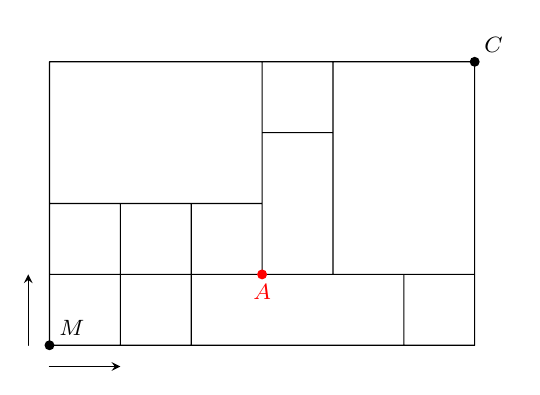
\begin{tikzpicture}[scale=0.9,>=stealth, font=\footnotesize, line join=round, line cap=round]
			\coordinate (M) at (0,0);
			\coordinate (A) at (3,1);
			\coordinate (C) at (6,4);
			\draw (M)node[above right]{$M$}--(6,0)--(C)node[above right]{$C$}--(0,4)--cycle (0,1)--(6,1) (0,2)--(3,2) (3,3)--(4,3) (1,0)--(1,2) (2,0)--(2,2) (A)node[below,red]{$A$}--(3,4) (4,1)--(4,4) (5,0)--(5,1);
			\draw[->] (-0.3,0)--(-0.3,1);
			\draw[->] (0,-0.3)--(1,-0.3);
			\fill[red] (A)circle(2pt);
			\fill (C)circle(2pt);
			\fill (M)circle(2pt);
		\end{tikzpicture}
	\end{center}
	Biết rằng toàn bộ cung đường theo bản đồ từ dưới lên trên và từ trái qua phải là đường một chiều vì vậy Mạnh chỉ được phép đi lên hoặc đi sang phải. Vậy Mạnh có bao nhiêu cách đến công ty?
	\shortans[oly]{$15$}
	\loigiai{
		Số cách Mạnh đến công ty là $15$ cách.\\
		Minh hoạ
		\begin{center}
			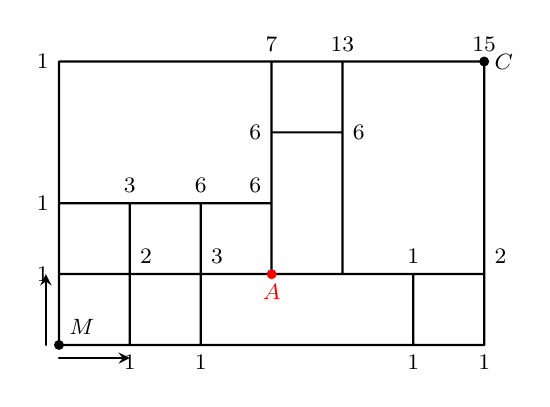
\begin{tikzpicture}[scale=0.9,>=stealth, font=\footnotesize, line join=round, line cap=round, thick]
				\coordinate (M) at (0,0);
				\coordinate (A) at (3,1);
				\coordinate (C) at (6,4);
				\draw (M)node[above right]{$M$}--(6,0)--(C)node[ right]{$C$}--(0,4)--cycle (0,1)--(6,1) (0,2)--(3,2) (3,3)--(4,3) (1,0)--(1,2) (2,0)--(2,2) (A)node[below,red]{$A$}--(3,4) (4,1)--(4,4) (5,0)--(5,1);
				\draw[->] (-0.185,0)--(-0.185,1);
				\draw[->] (0,-0.185)--(1,-0.185);
				\fill[red] (A)circle(2pt);
				\fill (C)circle(2pt);
				\fill (M)circle(2pt);
				\path 
				(1,0) node[below]{$1$} 			(2,0) node[below]{$1$} 
				(5,0) node[below]{$1$} 			(6,0) node[below]{$1$}
				(0,1) node[left]{$1$} 			(0,2) node[left]{$1$} 
				(0,4) node[left]{$1$}			(5,1) node[above]{$1$}
				(1,1) node[above right]{$2$} 	(6,1) node[above right]{$2$}
				(1,2) node[above]{$3$}			(2,1) node[above right]{$3$}
				(2,2) node[above]{$6$}			(3,2) node[above left]{$6$}
				(3,3) node[left]{$6$}			(4,3) node[right]{$6$}
				(3,4) node[above]{$7$}
				(4,4) node[above]{$13$}
				(6,4) node[above]{$15$}
				;
			\end{tikzpicture}
		\end{center}
	}
\end{ex}

\begin{ex}%[2D4V3-5]%Câu 4
	\immini[thm]{
		Bên trong hình vuông cạnh $4$, dựng hình sao bốn cạnh đều như hình vẽ bên (các kích thước cần thiết cho như ở trong hình vẽ).
		Tính thể tích $V$ của khối tròn xoay sinh ra khi quay hình sao đó quanh trục $Ox$ (làm tròn kết quả đến hàng phần mười).
	}{
		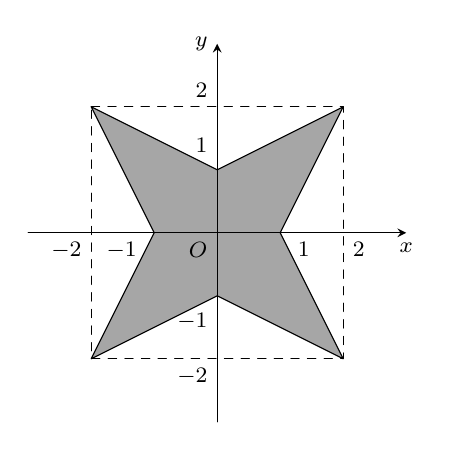
\begin{tikzpicture}[scale=0.8,>=stealth, font=\footnotesize, line join=round, line cap=round]
			\def\xmin{-3} \def\xmax{3}
			\def\ymin{-3} \def\ymax{3}
			\fill[gray!70] (-2,2)--(0,1)--(2,2)--(1,0)--(2,-2)--(0,-1)--(-2,-2)--(-1,0)--cycle;
			\draw[->] (\xmin,0)--(\xmax,0) node [below]{$x$};
			\draw[->] (0,\ymin)--(0,\ymax) node [left]{$y$};
			\node at (0,0) [below left]{$O$};
			\draw[dashed] (-2,2)--(2,2)--(2,-2)--(-2,-2)--cycle (-2,0)node[below left]{$-2$} (2,0)node[below right]{$2$} (0,2)node[above left]{$2$} (0,-2)node[below left]{$-2$};
			\draw (-2,2)--(0,1)node[above left,yshift=0.1cm]{$1$}--(2,2)--(1,0)node[below right,xshift=0.1cm]{$1$}--(2,-2)--(0,-1)node[below left,yshift=-0.1cm]{$-1$}--(-2,-2)--(-1,0)node[below left,xshift=-0.1cm]{$-1$}--cycle;
		\end{tikzpicture}
	}
	\shortans[0ly]{$20{,}9$}
	\loigiai{
		\begin{center}
			\begin{tikzpicture}[scale=1,>=stealth, font=\footnotesize, line join=round, line cap=round, thick, blue]
				\def\xmin{-3} \def\xmax{3} \def\ymin{-3} \def\ymax{3}
				\path 
					(-2,2) coordinate (A)
					(2,2) coordinate (B)
					(2,-2) coordinate (C)
					(-2,-2) coordinate (D)
					(0,1) coordinate (M)
					(1,0) coordinate (N)
					(0,-1) coordinate (P)
					(-1,0) coordinate (Q);
				\fill[gray!50] (-2,2)--(0,1)--(2,2)--(1,0)--(2,-2)--(0,-1)--(-2,-2)--(-1,0)--cycle;
				\draw[->] (\xmin,0)--(\xmax,0) node [below]{$x$};
				\draw[->] (0,\ymin)--(0,\ymax) node [left]{$y$};
				\node at (0,0) [below left]{$O$};
				\draw[dashed,thin] (-2,2)--(2,2)--(2,-2)--(-2,-2)--cycle (-2,0)node[below left]{$-2$} (2,0)node[below right]{$2$} (0,2)node[above left]{$2$} (0,-2)node[below left]{$-2$};
				\draw (-2,2)--(0,1)node[above left,yshift=0.1cm]{$1$}--(2,2)--(1,0)node[below right,xshift=0.1cm]{$1$}--(2,-2)--(0,-1)node[below left,yshift=-0.1cm]{$-1$}--(-2,-2)--(-1,0)node[below left,xshift=-0.1cm]{$-1$}--cycle;
				\foreach \x/\y in {A/135,B/45,C/-45,D/225,M/-45,N/225,P/45,Q/-45}
				\fill[black] (\x) circle (1pt) ($(\y:3mm)+(\x)$) node {$\x$};
			\end{tikzpicture}
		\end{center}
		Ta kí hiệu các điểm như hình vẽ.\\
		Ta có khối tròn xoay đó được tạo thành khi quay hình phẳng $QAMBN$ quanh trục $Ox$.\\
		Mà $S_{OQAM}=S_{ONBM}$ nên thể tích của khối tròn xoay đó sẽ bằng 2 lần thể tích của khối tròn xoay khi quay hình phẳng $ONBM$ quanh trục $Ox$.\\
		Suy ra ta có thể tích $V=2\left(\pi\displaystyle\int\limits_0^2 MB^2 \mathrm{\,d}x -\pi\displaystyle\int\limits_1^2 NB^2 \mathrm{\,d}x\right)$.
		\begin{itemize}
			\item[+)] Viết phương trình đường thẳng $MB$, với $M(0;1)$, $B(2;2)$.\\
			Có vectơ chỉ phương $\overrightarrow{MB}=(2;1)$ suy ra một vectơ pháp tuyến của đường thẳng là $\overrightarrow{n}_1=(-1;2)$.\\
			Suy ra $MB\colon -1\cdot(x-0)+2\cdot(y-1)=0 \Rightarrow -x+2y-2=0 \Rightarrow y=\dfrac{1}{2}x+1$.
			\item[+)] Tương tự, ta viết được phương trình đường thẳng $NB$ là\\
			$NB\colon -2\cdot(x-1)+1\cdot(y-0)=0 \Leftrightarrow -2x+y+2=0 \Rightarrow y=2x-2$
		\end{itemize}
		Thể tích là $V=2\left(\pi\displaystyle\int\limits_0^2 \left(\dfrac{1}{2}x+1\right)^2 \mathrm{\,d}x -\pi\displaystyle\int\limits_1^2 \left(2x-2\right)^2 \mathrm{\,d}x\right) =\dfrac{20}{3}\pi \approx 20{,}9$.
		}
\end{ex}

\begin{ex}%[2H2C2-6]%Câu 5
	Một ống phun nước có hình dạng như hình vẽ dưới. Để giữ cho ống nước được cân bằng không bị nghiêng kỹ sư sử dụng ba đoạn thép để nối các điểm $C$, $A$, $G$ với mặt đất, các đoạn thép $CD$, $GF$, $AE$ có độ lớn lực căng lần lượt bằng $1200$ N, $800$ N và $600$ N. Trong hệ tọa độ $Oxyz$, coi gốc tọa độ là chân ống nước, trục $Oz$ hướng lên trời, mặt đất là mặt phẳng $(Oxy)$ các thông số được cho như hình vẽ, đơn vị trên các hệ trục tọa độ tính bằng mét. Coi đường kính ống không đáng kể, độ lớn vectơ hợp lực của ba sợi thép tác động lên ông nước là bao nhiêu Newton (làm tròn kết quả đến hàng đơn vị).
	\begin{center}
		\includegraphics[scale=0.45]{images/de7-1}
	\end{center}
	\shortans[oly]{$2311$}
	\loigiai{
		Giả sử lực tác dụng lên 3 đoạn dây $CD$, $GF$, $AE$ lần lượt là $\overrightarrow{T}_1$, $\overrightarrow{T}_2$, $\overrightarrow{T}_3$.\\
		Suy ra hợp lực $\overrightarrow{T} =\overrightarrow{T}_1 +\overrightarrow{T}_2 +\overrightarrow{T}_3$ (*).\\
		(Áp dụng công thức: Cho 2 vec-tơ $\overrightarrow{u}$, $\overrightarrow{v}$ cùng hướng, ta có $\overrightarrow{u} =\dfrac{|\overrightarrow{u}|}{|\overrightarrow{v}|}\cdot\overrightarrow{v}$)
		\begin{enumerate}[+)]
			\item Vì $\overrightarrow{T_1}$ và $\overrightarrow{CD}$ cùng hướng nên ta suy ra $\overrightarrow{T_1}=\dfrac{T_1}{CD}\cdot\overrightarrow{CD}$.
			\item Vì $\overrightarrow{T_2}$ và $\overrightarrow{GF}$ cùng hướng nên ta suy ra $\overrightarrow{T_2}=\dfrac{T_2}{GF}\cdot\overrightarrow{GF}$.
			\item Vì $\overrightarrow{T_3}$ và $\overrightarrow{AE}$ cùng hướng nên ta suy ra $\overrightarrow{T_3}=\dfrac{T_3}{AE}\cdot\overrightarrow{AE}$.
		\end{enumerate}
		Suy ra $\overrightarrow{T} =\dfrac{T_1}{CD}\cdot\overrightarrow{CD} +\dfrac{T_2}{GF}\cdot\overrightarrow{GF} +\dfrac{T_3}{AE}\cdot\overrightarrow{AE}$.
		\begin{enumerate}[+)]
			\item Ta có $C(-1{,}5;0;4{,}5)$, $D(0;3;0)$ $\Rightarrow \overrightarrow{CD}=(1{,}5;3;-4{,}5) \Rightarrow CD=1{,}5\sqrt{14}$.
			\item Ta có $G(0;-1;3)$, $F(2;-1;0)$ $\Rightarrow \overrightarrow{GF}=(2;0;-3) \Rightarrow GF=\sqrt{13}$.
			\item Ta có $A(0;0;3)$, $E(-1{,}5;0;0)$ $\Rightarrow \overrightarrow{AE}=(-1{,}5;0;-3) \Rightarrow AE=1{,}5\sqrt{5}$.
		\end{enumerate}
		Suy ra 
		$\begin{aligned}[t]
			\overrightarrow{T} &=\dfrac{1\,200}{1{,}5\sqrt{14}}\cdot(1{,}5;3;-4{,}5) +\dfrac{800}{\sqrt{13}}\cdot(2;0;-3) +\dfrac{600}{1{,}5\sqrt{5}}\cdot(-1{,}5;0;-3) \\
			&=(496{,}145;641{,}427;-2164{,}437).
		\end{aligned}$\\
		Độ lớn của vec-tơ hợp lực là $|\overrightarrow{T}| =\sqrt{(496{,}145)^2+(641{,}427)^2+(-2164{,}437)^2} \approx 2311$.
	}
\end{ex}

\begin{ex}%[0H9C3-5]%Câu 6
	Hình vẽ sau mô tả một con thuyền đang kéo một người đàn ông trượt ván bằng một đoạn dây dài $9$ mét. Xét trên hệ trục $Oxy$ (đơn vị trên các hệ trục bằng mét), ban đầu con thuyền đang ở gốc tọa độ và di chuyển trên tia $Oy$, người đàn ông xuất phát từ điểm có tọa độ $(9;0)$ bị kéo theo và quãng đường di chuyển tạo thành một đường cong $y=f(x)$ (tham khảo hình vẽ dưới), bờ biển là đường thẳng $x+2y+1=0$. Khi người đàn ông đến gần bờ biển nhất thì khoảng cách giữa người đàn ông và trục $Oy$ bằng bao nhiêu mét (làm tròn kết quả đến hàng phần trăm)? Biết rằng trong quá trình di chuyển, người đàn ông luôn hướng về phía thuyền, đoạn dây luôn căng và nằm trên tiếp tuyến của đường cong $y=f(x)$.
	\begin{center}
		\includegraphics[scale=0.4]{images/de7-2}
	\end{center}
	\shortans[oly]{$8{,}05$}
	\loigiai{
%		\begin{center}
%			\includegraphics[scale=0.4]{images/de7-3}
%		\end{center}
	Giả sử người đó ở vị trí $M$, $M_0$ là điểm mà tiếp tuyến tại $M_0$ song song
	với đường thẳng $d\colon x+2y+1=0$.\\
	Dựng $M_0N\perp d$, $MK\perp d$.\\
	Dựa vào hình vẽ, ta có $MK\geq M_0N$ nên khoảng cách từ người đến bờ biển ngắn nhất khi tiếp tuyến tại $M$ song song với đường thẳng $x+2y+1=0$.\\
	Dựa vào hình, ta có
	\begin{enumerate}[+)]
		\item $\widehat{PM_0Q}=\widehat{PFO}$ (2 góc đồng vị)
		\item $\widehat{PFO}=\widehat{FED}$ (2 góc so le trong)
	\end{enumerate}
	Suy ra $\widehat{PM_0Q}=\widehat{FED}$.\\
	Thay lần lượt $x=0, y=0$ vào đường thẳng $x+2y+1=0$, ta có $E(-1;0)$, $D\left(0;\frac{1}{2}\right)$ $\Rightarrow \heva{&OE=1\\ &OD=\dfrac{1}{2}.}$\\
	Xét tam giác vuông $OED$, ta có $\tan\widehat{OED}=\dfrac{OD}{OE}=\dfrac{\frac{1}{2}}{1} =\dfrac{1}{2} \Rightarrow \widehat{OED}=\widehat{PM_0Q}\approx26{,}565^\circ$.\\
	Xét tam giác vuông $PM_0Q$, ta có $$\cos\widehat{PM_0Q}=\dfrac{QM_0}{PM_0} \Rightarrow QM_0=\cos\widehat{PM_0Q}\cdot PM_0 =9\cdot\cos(26{,}565^\circ)\approx8{,}05\, (\rm m).$$
	}
\end{ex}
\Closesolutionfile{ans}

\inputansbox{3}{ans/de7-KQ}